\chapter{Integración}
\section{Elementos de integración numérica}
A menudo surge la necesidad de evaluar la integral definida de una fucnión que no tiene una antiderivada o cuta antiderivada no es fácil de obtemer. El método básico asociado con la aproximación de $\int_{a}^{b} f(x) dx$ recibe el nombre de cuadratura numérica. Éste utiliza una suma $\sum_{i = 0}^{n} a_i f(x_i)$ para aproximar $\int_{a}^{b} f(x) dx$.

Los métodos de cuadratura se basan en los polinomios de interpolación. La idea básica es seleccionar un conjunto de nodos distintos $\{x_0, ..., x_n\}$ del intervalo $[a, b]$. Entonces integramos el polinomio interpolante de Lagrange
\[ P_n(x) = \sum_{i = 0}^{n} f(x_i) L_i(x) \]
y su término de error de truncamiento sobre $[a, b]$ para obtener
\begin{multline*}
    \resizebox{0.45 \textwidth}{!}{$
    \int_{a}^{b} f(x) dx = \int_{a}^{b} \sum_{i = 0}^{n} f(x_i) L_i(x) dx + \int_{a}^{b} \prod_{i = 0}^{n} (x - x_i) \frac{f^{(n + 1)} (\xi(x))}{(n + 1)!} dx
    $} \\
    \resizebox{0.45 \textwidth}{!}{$
    = \sum_{i = 0}^{n} a_i f(x_i) + \frac{1}{(n + 1)!} \int_{a}^{b} \prod_{i = 0}^{n} (x - x_i) f^{(n + 1) (\xi(x)) dx}
    $} 
\end{multline*}
donde $\xi(x)$ se encuentra en $[a, b]$ para cada $x$ y
\[ a_i = \int_{a}^{b}L_i(x)dx, \text{ para cada } i = 0, 1,..., n\]
La fórmula de cuadratura es, por lo tanto,
\[ \int_{a}^{b} f(x) dx  \approx \sum_{i = 0}^{n} a_i f(x_i) \]
con un error dado por 
\[ E(f) = \frac{1}{(n + 1)!} \int_{a}^{b} \prod_{i = 0}^{n} (x - x_i) f^{(n + 1)} (\xi(x)) dx\]

Antes de analizar la situación general de las fórmulas de cuadratura, consideremos las fórmulas producidas mediante el uso del primer y del segundo polinomios de Lagrange con nodos igualmente espaciados. Esto da la regla trapezoidal y la regla de Simpson.

\subsection{La regla trapezoidal}
Para derivar la regla trapezoidal (o regla del trapecio) para aproximar $\int_{a}^{b} f(x) dx$, sean $x_0 = a$, $x_1 = b$, $h = b - a$ y utilice el polinomio de Lagrange
\[ P_1(x) = \frac{(x - x_1)}{(x_0 - x_1)} f(x_0) + \frac{(x - x_0)}{(x_1 - x_0)} f(x_1) \]
Entonces
\begin{multline}
    \label{eq: Burden 4.23}
    \int_{a}^{b} f(x) dx = \int_{x_0}^{x_1} \left[ \frac{(x - x_1)}{x_0 - x_1} f(x_0) + \frac{(x - x_0)}{(x_1 - x_0)} f(x_1) \right] dx \\
    + \frac{1}{2} \int_{x_0}^{x_1} f''(\xi(x)) (x - x_0) (x - x_1) dx
\end{multline}
El producto $(x - x_0) (x - x_1)$ no cambia de signo en $[x_0, x_1]$, por lo que el teorema de valor promedio ponderado para integrales se puede aplicar al término de error para obtener, para algunos $\xi$ en $(x_0, x_1)$,
\begin{align*}
    & \int_{x_0}^{x_1} f''(\xi(x)) (x - x_0) (x - x_1) dx \\
    & = f''(\xi) \int_{x_0}^{x_1} (x - x_0) (x - x_1) dx \\
    & = f''(\xi) \left[ \frac{x^3}{3} - \frac{(x_1 + x_0)}{2}x^2 + x_0 x_1 x \right]_{x_0}^{x_1} \\
    & = - \frac{h^3}{6} f''(\xi)
\end{align*}
Por consiguiente, la ecuación \ref{eq: Burden 4.23} implica que
\begin{align*}
    & \int_{a}^{b} f(x) dx = \\
    & = \left[ \frac{(x - x_1)^2}{2 (x_0 - x_1)} f(x_0) + \frac{(x - x_0)^2}{2(x_1 - x_0)} f(x_1) \right]_{x_0}^{x_1} - \frac{h^3}{12} f''(\xi) = \\
    & = \frac{(x_1 - x_0)}{2} [f(x_0) + f(x_1)] - \frac{h^3}{12} f''(\xi)
\end{align*}
Por medio de la notación $h = x_1 - x_0$ obtenemos la siguiente regla:
\subsubsection{Regla trapezoidal:}
\[ \int_{a}^{b} f(x) dx = \frac{h}{2} [f(x_0) + f(x_1)] - \frac{h^3}{12} f''(\xi) \]

Esto recibe el nombre de regla trapezoidal porque cuando $f$ es una función con valores positivos, $\int_{a}^{b}f(x) dx$ se aproxima mediante el área de un trapecio, como se muestra en la figura \ref{fig: Regla del Trapecio}

\begin{figure}[h]
    \centering
    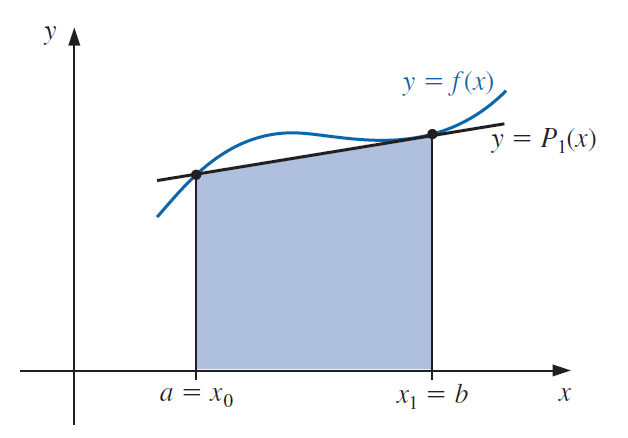
\includegraphics[width = 0.5 \textwidth]{Imagenes/5 - Regla del Trapecio.png}
    \caption{Regla del Trapecio.}
    \label{fig: Regla del Trapecio}
\end{figure}

El término de error para la regla trapezoidal implica $f''$, por lo que la regla da el resultado exacto cuando se aplica a cualquier función cuya segunda derivada es idénticamente cero, es decir, cualquier polinomio de grado uno o menos.

\subsection{Regla de Simpson}
La regla de Simpson resulta de la integración sobre $[a, b]$ del segundo polinomio de Lagrange con nodos igualmente espaciados $x_0 = a$, $x_2 = b$ y $x_1 = a + h$, en donde $h = (b - a)/2$ (véase la figura \ref{fig: Regla de Simpson}).

\begin{figure}[h]
    \centering
    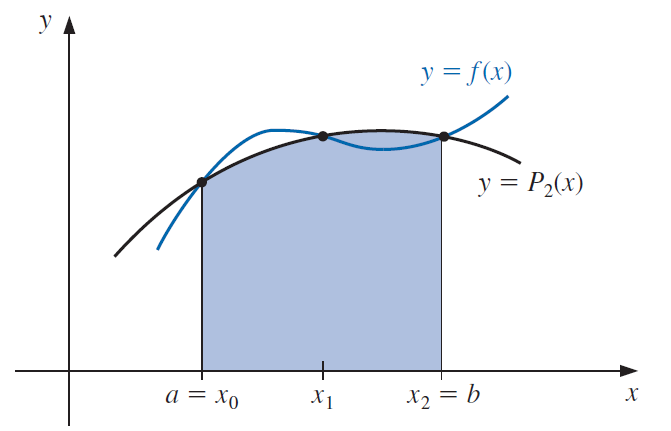
\includegraphics[width = 0.5 \textwidth]{Imagenes/5 - Regla de Simpson.png}
    \caption{Regla de Simpson.}
    \label{fig: Regla de Simpson}
\end{figure}
Por lo tanto,
\begin{align*}
    & \int_{a}^{b} f(x) dx = \int_{x_0}^{x_2} \left[ \frac{(x - x_1)(x - x_2)}{(x_0 - x_1)(x_0 - x_2)} f(x_0) + \right. \\ 
    & \left. \frac{(x - x_0)(x - x_2)}{(x_1 - x_0)(x_1 - x_2)} f(x_1) + \frac{(x - x_0)(x - x_1)}{(x_2 - x_0)(x_2 - x_1)} f(x_2) \right] dx \\
    & + \int_{x_0}^{x_2} \frac{(x - x_0)(x - x_1) (x - x_2)}{6} f^{(3)} (\xi(x)) dx
\end{align*}
Al deducir la regla de Simpson de esta forma, sin embargo, da un solo término de error $O(h^4)$ relacionado con $f^{(3)}$. Al aproximar el problema de otra forma, se puede derivar otro término de orden superior relacionado con $f^{(4)}$.

Para ilustrar este método alternativo, suponga que $f$ se expande en el tercer polinomio de Taylor alrededor de $x_1$. Entonces, para cada $x$ en $[x_0, x_2]$, existe un número $\xi(x)$ en $(x_0, x_2)$ con
\begin{align*}
    & f(x) = f(x_1) + f'(x_1) (x - x_1) + \frac{f''(x_1)}{2} (x - x_1)^2 \\
    & + \frac{f'''(x_1)}{6} (x - x_1)^3 + \frac{f^{(4)} (\xi(x))}{24} (x - x_1)^4
\end{align*}
y
\begin{align}
    \label{eq: Burden 4.24}
    & \int_{x_0}^{x_2} f(x) dx = \left[ f(x_1) (x - x_1) + \frac{f'(x_1)}{2} (x - x_1)^2 \right. \notag \\
    & \left. \frac{f''(x_1)}{6} (x - x_1)^3 + \frac{f'''(x_1)}{24} (x - x_1)^4 \right]_{x_0}^{x_2} \\
    & + \frac{1}{24} \int_{x_0}^{x_2} f^{(4)}(\xi(x)) (x - x_1)^4 dx \notag
\end{align}
Puesto que $(x - x_1)^4$ nunca es negativo en $[x_0, x_2]$, el teorema de valor promedio ponderado para las integrales implica que 
\begin{align*}
    & \frac{1}{24} \int_{x_0}^{x_2} f^{(4)} (\xi(x)) (x - x_1)^4 dx = \\
    & = \frac{f^{(4)}(\xi_1)}{24} \int_{x_0}^{x_2} (x - x_1)^4 dx = \left. \frac{f^{(4)}(\xi_1)}{120}(x - x_1)^5 \right]_{x_0}^{x_2}
\end{align*}
para algún número $\xi_1$ en $(x_0 , x_2)$.

Sin embargo, $h = x_2 - x_1 = x_1 - x_0$, por lo que 
\[ (x_2 - x_1)^2 - (x_0 - x_1)^2 = (x_2 - x_1)^4 - (x_0 - x_1)^4 = 0 \]
mientras
\[ (x_2 - x_1)^3 - (x_0 - x_1)^3 = 2h^3 \text{ y } (x_2 - x_1)^5 - (x_0 - x_1)^5 = 2h^5\]
Por consiguiente, la ecuacion \ref{eq: Burden 4.24} se puede escribir como 
\[ \int_{x_0}^{x_2} f(x) dx = 2h f(x_1) + \frac{h^3}{3} f''(x_1) + \frac{f^{(4)}(\xi_1)}{60} h^5 \]

Ahora, si reemplazamos $f''(x_1)$ por medio de la aproximación determinada en la ecuación \ref{Eq: (9.3)} de la sección 1 del capítulo 2, tenemos
\begin{align*}
    & \int_{x_0}^{x_2} f(x) dx = 2 h f(x_1) + \frac{h^3}{3} \left\{ \frac{1}{h^2} [f(x_0) - 2 f(x_1) + f(x_2)] \right. \\
    & \left. - \frac{h^2}{12} f^{(4)} (\xi_2) \right\} + \frac{f^{(4)}(\xi_1)}{60} h^5 = \\
    & = \frac{h}{3} [f(x_0) + 4f(x_1) + f(x_2)] - \frac{h^5}{12} \left[ \frac{1}{3} f^{(4)}(\xi_2) - \frac{1}{5} f^{(4)}(\xi_1) \right]
\end{align*}

Con métodos alternos se puede mostar que los valores $\xi_1$ y $\xi_2$ en esta expresión se pueden reemplazar mediante un valor común $\xi$ en $(x_0, x_2)$. Esto da la regla de Simpson.

\subsubsection{Regla de Simpson:}
\[ \int_{x_0}^{x_2} f(x) dx = \frac{h}{3} [f(x_0) + 4 f(x_1) + f(x_2)] - \frac{h^5}{90} f^{(4)}(\xi)\]

El término de error en la regla de Simpson implica la cuarta derivada de $f$, por lo que da resultados exactos cuando se aplica a cualquier polinomio de grado tres o menos.

\subsection{Precisión de medición}
Las derivadas estándar de las fórmulas de error de cuadratura están basadas al determinar la clase de polinomios para los que estas fórmulas producen resultados exactos. La siguiente definición se utiliza para facilitar el análisis de esta derivada.

\begin{definition}
    El grado de precisión, o precisión, de una fórmula de cuadratura es el mayor entero positivo $n$, de tal forma que la fórmula es exacta para $x^k$, para cada $k = 0,1...,n$.
\end{definition}

Esta definición implica que las reglas trapezoidal y de Simpson tienen grados de precisión uno y tres, respectivamente.

\section{Integración numérica compuesta}

\begin{theorem}
    Si $f \in C^4[a, b]$, $n$ es par, $h = (b - a)/n$, y $x_j = a + jh$, para cada $j = 0, 1,..., n$. Existe $\mu \in (a, b)$ para los que la regla compuesta de Simpson para $n$ subintervalos se puede reescribir con su término de error como
    \begin{align*}
        & \int_{a}^{b} f(x) dx = \frac{h}{3} \left[ f(a) + 2 \sum_{j = 1}^{(n/2)-1} f(x_{2j}) \right. \\
        & \left. + 4 \sum_{j = 1}^{n/2} f(x_{2j} - 1) + f(b) \right] - \frac{b - a}{180} h^4 f^{(4)} (\mu)
    \end{align*}
\end{theorem}

Observe que el término de error para la regla compuesta de Simpson es $O(h^4)$, mientras que era $O(h^5)$ para la regla estándar de Simpson. Sin embargo, estos índices no son comparables ya que para la regla estándar de Simpson, tenemos $h$ fija en $h = (b - a)/2$, pero para la regla compuesta de Simpson, tenemos $h = (b - a)/n$, para $n$ un entero par. Esto nos permite reducir considerablemente el valor de $h$.

El enfoque de subdivisión se puede aplicar a cualquiera de las fórmulas de Newton-Cotes. Las extensiones de las reglas trapezoidal y de punto medio se dan sin prueba. La regla trapezoidal sólo requiere un intervalo para cada aplicación, por lo que el entero $n$ puede ser tanto par como impar.

\begin{theorem}
    Sean $f \in C^2[a, b]$, $h = (b- a)/n$, y $x_j = a + jh$, para cada $j = 0,1,...,n$. Existe $\mu \in (a, b)$ para el que la regla compuesta trapezoidal para $n$ subintervalos se puede reescribir con este término de error como 
    \[ \int_{a}^{b} f(x) dx = \frac{h}{2} \left[ f(a) + 2 \sum_{j = 1}^{n - 1}f(x_j) + f(b) \right] - \frac{b - a}{12} h^2 f''(\mu) \]
\end{theorem}

\section*{Ejercicios}
\noindent (1) Calcular $\int_{0}^{1} \frac{2}{x^2 + 4}$ utilizando:
\begin{itemize}
    \item La regla del trapecio de Simpson simples
    \item La regla compuesta del trapecio con $h = 1/2^k$, $k = 2,...,6$
    \item La regla compuesta de Simpson con $h = 1/2^k$, $k = 2,...,6$
\end{itemize}

\noindent (2) Aproxime $\int_{0}^{1} x^3 dx$ usando la regla compuesta del trapecio eligiendo el valor de $h$ adecuado para que el error sea menor que $\delta = 10^-6$.

\noindent (3) Sea $f : [0, 1] \rightarrow \mathbb{R}$, se considera la fórmula de cuadratura
\[ Q[f] = af(1/4) + bf(1/2) + cf(3/4) \]
para aproximar $\int_{0}^{1} f(x) dx$, se pide:
\begin{itemize}
    \item determinar los valors constantes $a$, $b$, y $c$ de modo que la fórmula de cuadratura $Q[f]$ tenga grado de exactitud máximo.
    \item Aplicar la fórmula obtenida para aproximar
    \[ \int_{0}^{1} \frac{x^2}{\sqrt{x^2 + 12}} dx \]
\end{itemize}

\noindent (4) De una fuerza $F(x)$ que depende de la posición $x$, contamos con las siguientes mediciones discretas a intervalor de 5 m.
\[ x(m): 0 \quad 5 \quad 10 \quad 15 \quad 20 \]
\[ F(N): 0 \quad 1.53 \quad 9.51 \quad 8.70 \quad 2.81 \]
\begin{itemize}
    \item estimar el valor de $F$ para un valor de $x = 6m$ utilizando un polinomio interpolador cuadrátivo
    \item estimar el trabajo realizado por la fuerza
    \[ W = \int_{0}^{20} F(x) dx \]
    utilizando la regla de los trapecios compuestas y la regla de Simpson compuesta.
\end{itemize}